% Unofficial UChicago CS Poster Template
% v1.1.0 released September 8, 2022
% https://github.com/k4rtik/uchicago-poster
% a fork of https://github.com/anishathalye/gemini

\documentclass{beamer}

% ====================
% Packages
% ====================

\usepackage[T1]{fontenc}
\usepackage{lmodern}
\usepackage[size=custom,width=120,height=80,scale=1.0]{beamerposter}
\usetheme{gemini}
\usecolortheme{uchicago}
\usepackage{graphicx}
\usepackage{booktabs}
\usepackage{doi}
\usepackage[numbers]{natbib}
\usepackage[patch=none]{microtype}
\usepackage{tikz}
\usepackage{pgfplots}
\pgfplotsset{compat=1.18}
\usepackage{anyfontsize}
\usepackage{subcaption}

\pdfstringdefDisableCommands{%
\def\translate#1{#1}%
}

% ====================
% Lengths
% ====================

% If you have N columns, choose \sepwidth and \colwidth such that
% (N+1)*\sepwidth + N*\colwidth = \paperwidth
\newlength{\sepwidth}
\newlength{\colwidth}
\setlength{\sepwidth}{0.025\paperwidth}
\setlength{\colwidth}{0.3\paperwidth}

\newcommand{\separatorcolumn}{\begin{column}{\sepwidth}\end{column}}

% ====================
% Title
% ====================

\title{Learning Renormalization Group Flows of Ising Models}

\author{Jay Shen \inst{1} \and Ying-Jer Kao \inst{2} \and Wanda Hou \inst{3} \and Yi-Zhuang You \inst{3}}

\institute[shortinst]{\inst{1} University of Chicago \samelineand \inst{2} National Taiwan University \samelineand \inst{3} UC San Diego}

% ====================
% Footer (optional)
% ====================

\footercontent{
  \href{https://github.com/jshe2304/dlrg}{https://github.com/jshe2304/dlrg}
  \hfill
  Midwest Thermodynamics and Statistical Mechanics Conference 2025
  \hfill
  \href{mailto:alyssa.p.hacker@example.com}{jshe@uchicago.edu}}
% (can be left out to remove footer)

% ====================
% Logo (optional)
% ====================

% use this to include logos on the left and/or right side of the header:
% \logoright{\includegraphics[height=7cm]{logo1.pdf}}
% \logoleft{\includegraphics[height=7cm]{logo2.pdf}}

% ====================
% Body
% ====================

\begin{document}

\begin{frame}[t]
\begin{columns}[t]
\separatorcolumn

\begin{column}{\colwidth}

    \begin{block}{Introduction}

    Real space renormalization is a theoretically powerful but practically difficult technique for investigating scale and phase behavior in physical systems. For even the simplest problems, formulating the so-called renormalization group (RG) flow is incredibly difficult but, once accurately described, incredibly useful. Hou et al. proposed the MLRG method which approximates RG flows of Ising models automatically using neural networks. Here, we refine their algorithm, discuss its design space, and demonstrate some successes and limitations. 
    
    \end{block}
    
    \begin{block}{Theory}
    
    The isotropic homogenous Ising model is a graph with $N$ nodes $\sigma_i \in \{-1, 1\}$ and adjacency list $\mathcal{E}$, with $(i, j) \in \mathcal{E}$ indicating $\sigma_i$ and $\sigma_j$ are neighboring nodes on the lattice. The values of neighboring $\sigma_i$ and $\sigma_j$ correlated according to coupling constant $J$. 
    
    A renormalization transformation defines a coarse-grained lattice (primed) with $N' < N$ nodes and solves for the coupling constant $J'$ which best matches the fine-grained system's behavior: 
    
    \[
    H = - J \sum_{(i, j) \in \mathcal{E}} \sigma_i \sigma_j 
    \quad \Rightarrow \quad 
    H' = - J' \sum_{(i, j) \in \mathcal{E}'} \sigma_i \sigma_j
    \]
    \begin{figure}
        \centering
        
\includegraphics[width=0.6\linewidth]{figures/lieb-blocking.png}
    \end{figure}

    In principle, there exists a function $f$, called the renormalization group flow, which maps fine-grained coupling constants $J$ to coarse-grained coupling constants $J'$ by predicting the difference $f(J) = J' - J$:
    
    Rather than deriving this $f$ analytically, we learn an approximation $f_\theta(J)$ using a neural network. The neural network parameters are adjusted to minize the KL divergence between Ising model Gibbs distributions: 
    
    \[
    \text{Loss} = D_{KL} \bigg( \: \frac{1}{Z} e^{H(J)} \: \bigg|\bigg| \:\frac{1}{Z'} e^{H'(f_\theta(J) + J))}\bigg)
    \]

    \end{block}

\end{column}

\separatorcolumn

\begin{column}{\colwidth}

    \begin{block}{The Improved MLRG Algorithm}
        \begin{enumerate}
            \item{
                \textbf{Sample values of $J$}
        
                Hamiltonian Monte Carlo (HMC) \cite{betancourt-hmc, duane-hmc} is used to refine the zeros (critical points) of $f_\theta$ by sampling from the unnormalized probability distribution:
                
                \[
                    \tilde{P}(J) = \exp \big[- \alpha J ^2 - \beta || f_\theta(J) ||^2 \: \big]
                \]
                
                For stability, the potential is annealed in during training by increasing $\beta$ from $0$ to some $\beta_T$ and decreasing $\alpha$ from $\alpha_0$ to $0$. 
            }
            \item{
                \textbf{Forward pass to get $J'$}
                
                \[
                J' = J + f_\theta(J)
                \]
            }
            \item {
                \textbf{Evaluate the error}
        
                We implement the Ising lattices as Restricted Boltzmann Machines (RBMs) with visible and hidden spins, allowing for easy definition of the renormalization transformation and the appropriate KL divergence. 
                
                We use the common contrastive approximation for the loss:
                
                \[
                    D_{KL} \bigg( \: \frac{1}{Z} e^{H(J)} \: \bigg|\bigg| \:\frac{1}{Z'} e^{H'(f_\theta(J) + J))}\bigg) \approx F_{coarse}(\vec{v}_{fine}) - F_{coarse}(\vec{v}_{coarse})
                \]
                
                Here, $F_{coarse}$ is the free energy function of the coarse-grained RBM and $\vec{v}_{fine}$ and $\vec{v}_{coarse}$ are visible spins Gibbs-sampled from the fine and coarse-grained RBMs, respectively. 
            }
            
            \item{
                \textbf{Backpropagate error to $\theta$}

                Both the contrastive and the full KL losses are composed functions of $f_\theta(J)$, so we can backpropagate to adjust the parameters $\theta$. 
            }
            
        \end{enumerate}

        \begin{block}{Notable Elements of the Algorithmic Space}
            \begin{itemize}
                \item{
                    Hou et al. learn the C-theorem monotone $C(J)$, whereas we learn $f(J) = \nabla C(J)$, which is substantially faster. 
                }
                \item{
                    Hou et al. use higher-order spins to obtain better critical point estimates. We adopt this approach, and show that it is compatible with our other modifications. 
                }
                \item{
                    For small lattices, the KL-divergence is tractable to compute but mitigates only variance not bias. 
                }
                \item{
                    For training stability, we find the number of fine-grained Gibbs steps and the number of HMC trajectories should be above some threshold. Tuning hyperparameters is minimally effective. 
                }
            \end{itemize}
            
        \end{block}
    \end{block}

\end{column}

\separatorcolumn

\begin{column}{\colwidth}

    \begin{block}{Results}

    \begin{figure}
        \centering
        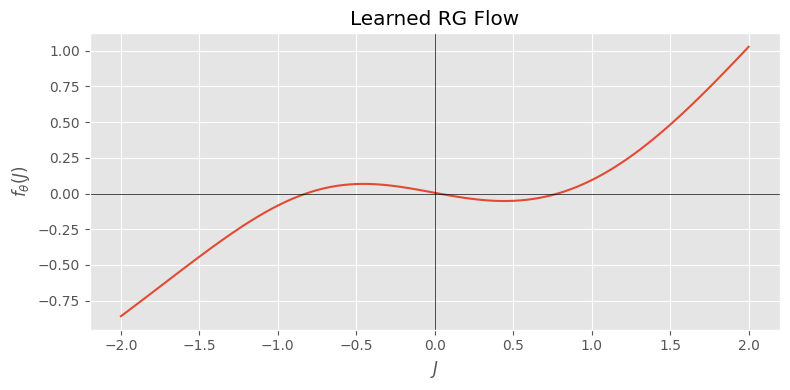
\includegraphics[width=0.6\linewidth]{figures/a1-flow.png}
    \end{figure}
    
    Training to convergence yields a flow with expected properties of odd parity, fixed points at $0$ and $\pm \infty$, and a pair of finite critical points. 
    
    \begin{figure}
        \centering
        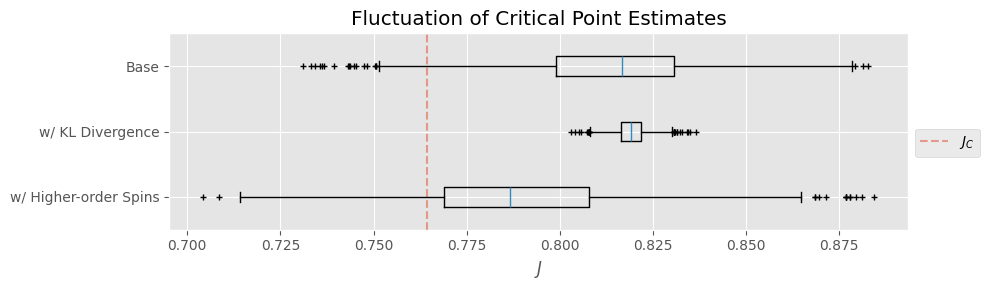
\includegraphics[width=0.7\linewidth]{figures/estimates.png}
    \end{figure}
    
    We obtain estimates close to the actual critical point. Using the KL divergence and higher-order spins can achieve improvements in variance and bias, respectively. 
    
    \begin{figure}
        \centering
        \begin{subfigure}[t]{0.5\textwidth}
            \centering
            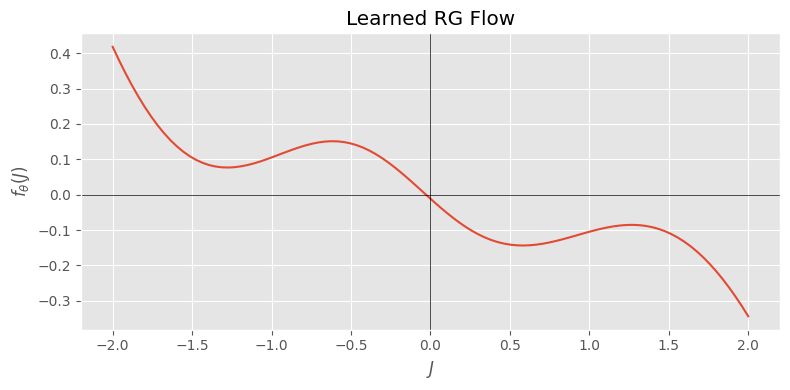
\includegraphics[width=\linewidth]{figures/a1-flow-2.png}
            \caption{Two-block Lieb lattice}
        \end{subfigure}%
        \begin{subfigure}[t]{0.5\textwidth}
            \centering
            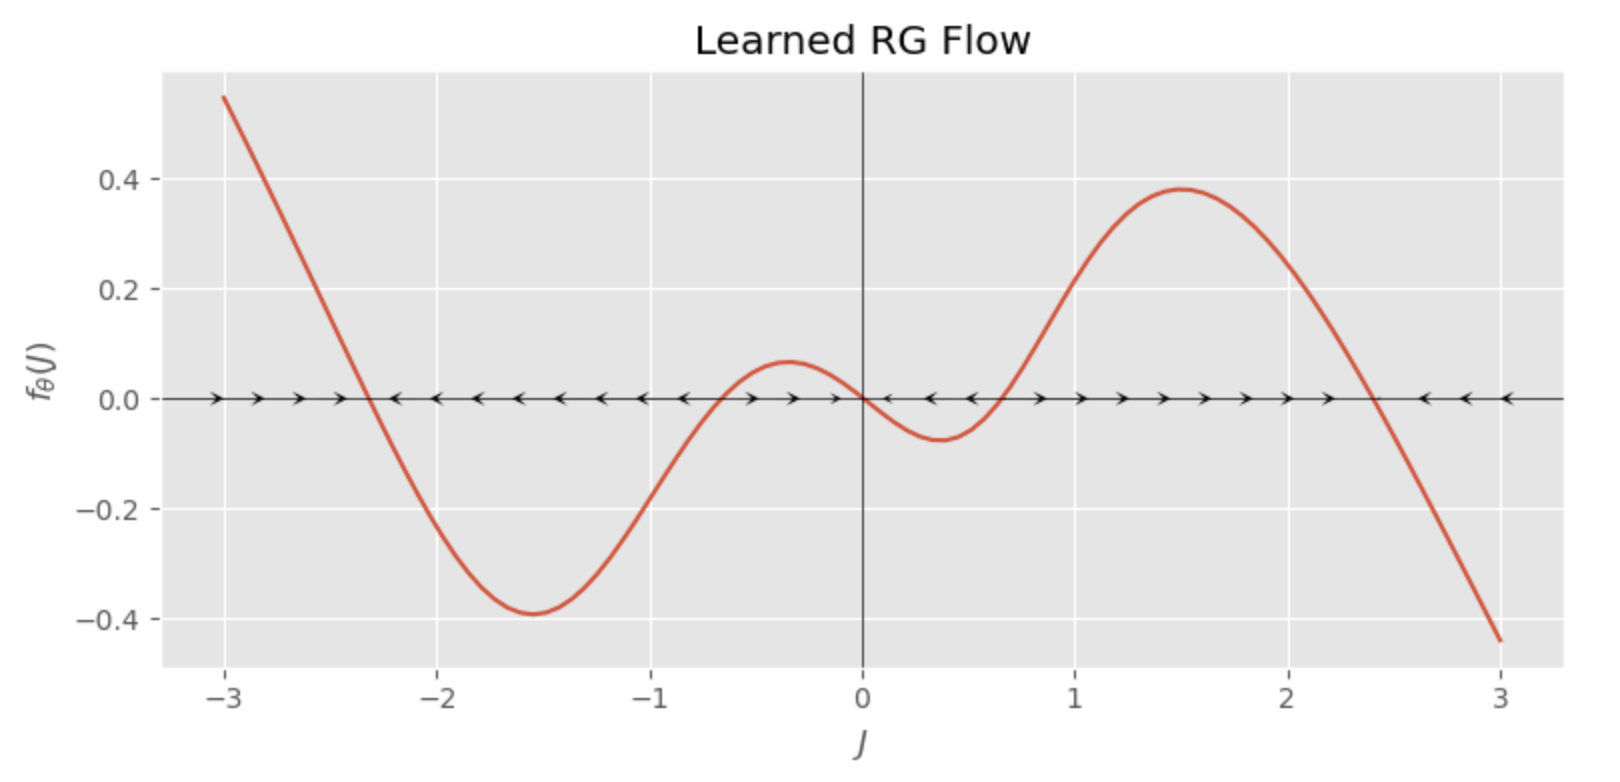
\includegraphics[width=\linewidth]{figures/a1-flow-3.png}
            \caption{Three-block Lieb lattice}
        \end{subfigure}
    \end{figure}
    
    The MLRG approach is limited in that it does not learn the same flows for lattices that should, in principle, be thermodynamically identical. 
    
    It is interesting to note that there appears to be an even-odd effect among learned flows—the algorithm finds critical points only for odd lattices. 

    \end{block}
    
    
    \begin{block}{References}
    
    \nocite{*}
    \footnotesize{\bibliographystyle{plainnat}\bibliography{poster}}
    
    \end{block}

\end{column}

\separatorcolumn
\end{columns}
\end{frame}

\end{document}